\documentclass{article}
\usepackage[utf8]{inputenc}
\usepackage{amsmath, amsthm, amsfonts,amssymb}
\usepackage[spanish]{babel}
\usepackage{multicol}
\usepackage{listings}
\lstset{basicstyle=\footnotesize\ttfamily,breaklines=true}
\usepackage{alltt}
\usepackage{graphicx}
\usepackage{subfigure}
\usepackage{subfig}
\usepackage{float}
\usepackage{url}
\usepackage{enumerate}
\usepackage{color}
\usepackage{cancel}
\usepackage{wrapfig}\definecolor{shadecolor}{RGB}{250,250,250}
\usepackage{framed}
\usepackage{epstopdf}
\setlength\parindent{0pt}
\usepackage{listings}
\usepackage{color} %red, green, blue, yellow, cyan, magenta, black, white
% Operadores matemáticos y simbolos
\DeclareMathOperator{\dive}{div}
\DeclareMathOperator{\trace}{trace}
\DeclareMathOperator{\tr}{tr}
\DeclareMathOperator{\symm}{symm}
\DeclareMathOperator{\sk}{skew}
\DeclareMathOperator{\grad}{grad}
\DeclareMathOperator{\Grad}{Grad}
\DeclareMathOperator{\curl}{curl}
\DeclareMathOperator{\Curl}{Curl}
\def\R{\mbox{\(\mathbb{R}\)}}
\def\E{\mbox{\(\mathbb{E}\)}}
\def\P{\mbox{\(\mathbb{P}\)}}
\def\I{\mbox{\(\mathbb{I}\)}}
\def\L{\mbox{\(\mathbb{L}\)}}
\def\dx{\mbox{\(\,\mathrm{d}x\)}}
\usepackage{changepage}
\usepackage[showframe=false]{geometry}
\geometry{left=2.5cm, right=2.5cm, top=2cm, bottom=3cm}
\title{Tarea 4\\}
\author{Luis Felipe Silva De Vidts}
\begin{document}
\begin{figure}
\begin{minipage}{2.5cm}

\includegraphics[width=0.8\textwidth]{./figures/LogoUC-BN}
\end{minipage}
\begin{minipage}{14.5cm}
\vspace{4mm}
{\sc PONTIFICIA UNIVERSIDAD CAT\'OLICA DE CHILE}\\
Facultad de Matemáticas\\
Departamento de Estadísica\\
{\bf EYP1113 Probabilidades y Estadística}\\
\vspace{0mm}
\hrulefill
\end{minipage}
\end{figure}
\phantom{""}
\vspace{-5mm}
\normalsize
\begin{center}
\Huge Tarea 1\\
\normalsize Luis Felipe Silva De Vidts
\end{center}
\section*{Parte I}
\begin{figure}[h!]
\centering
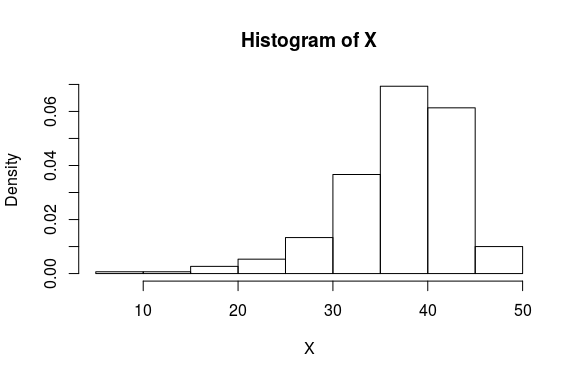
\includegraphics[scale=0.8]{./figures/hist_X.png}
\caption{Histograma de Datos01.txt}
\end{figure}
\begin{figure}[h!]
\begin{minipage}{6cm}
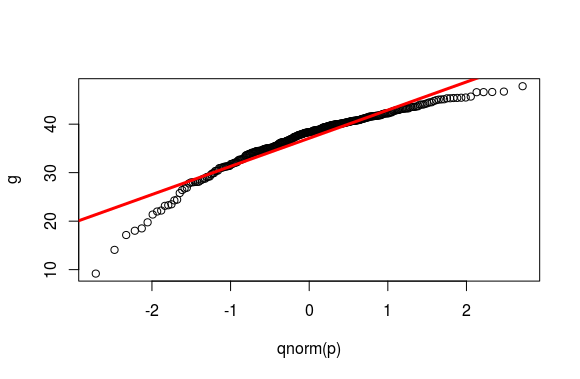
\includegraphics[scale=0.5]{./figures/normal.png}
\caption{QQ-plot de normal}
\end{minipage}
\hspace*{2cm}
\begin{minipage}{6cm}
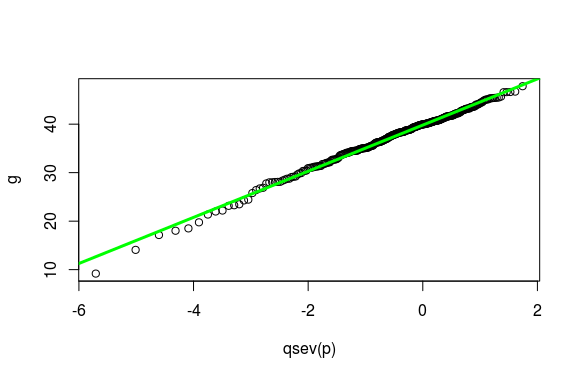
\includegraphics[scale=0.5]{./figures/sev.png}
\caption{QQ-plot de SEV}
\end{minipage}
\end{figure}
\begin{figure}[h!]
\centering
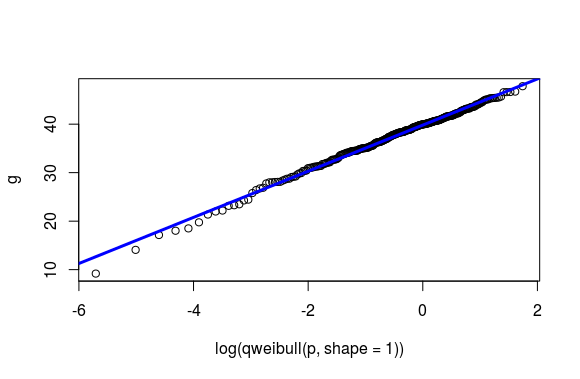
\includegraphics[scale=0.5]{./figures/weibull.png}
\caption{QQ-plot de Weibull}
\end{figure}
Como notamos en los gráficos anteriores los casos de Weibull y SEV parecen tener un mejor ajuste a los datos. Por lo que comparamos que tan bueno es la aproximacion de forma visual al ajustarlos al histograma de los datos las distribuciones anteriores
\begin{figure}[h!]
\centering
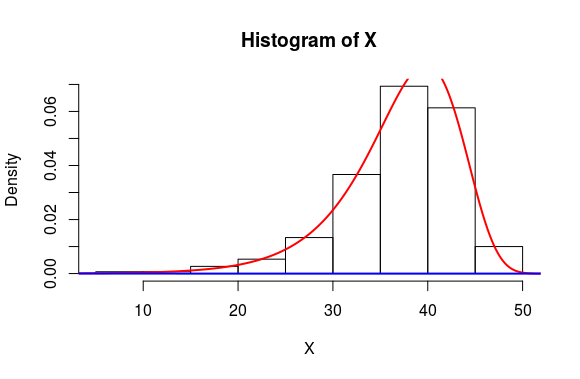
\includegraphics[scale=0.5]{./figures/sev_vs_weibull.png}
\caption{SEV(rojo) vs Weibull(azul)}
\end{figure}
En este caso tome los valores de la Weibull suponiendo que la recta entregada al hacer los QQ-plot era de la forma:
$$\ln(x)=\ln(b)+\frac{1}{a}\ln(-\ln(1-F(x))) $$
donde $F(x)$ es la función de densidad acumulada de la Weibull, donde obtuve que $b=1.956294e+17$ y $a =0.2102157$. \\

Por otro lado los de SEV suponiendo que la recta era:
$$x=\mu+\sigma\ln(-\ln(1-F(x))) $$
obteniendo $\mu = 39.815 $ y $\sigma=4.757018$\\

\pagebreak
\begin{figure}[h!]
\centering
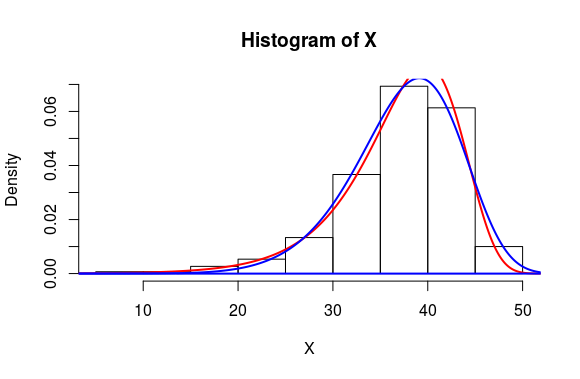
\includegraphics[scale=0.5]{./figures/version2.png}
\caption{Ajustando Weibull mediante método de momentos}
\end{figure}
Dado que el gráfico anterior no me parece representativo de la realidad utilice el método de los momentos para estimar los parámetros de la Weibull y obtuve que $a\approx 7.757018$ y $b\approx 40$, obteniendo el siguiente gráfico, que se asemeja a lo esperado.\\

\begin{figure}[h!]
\centering
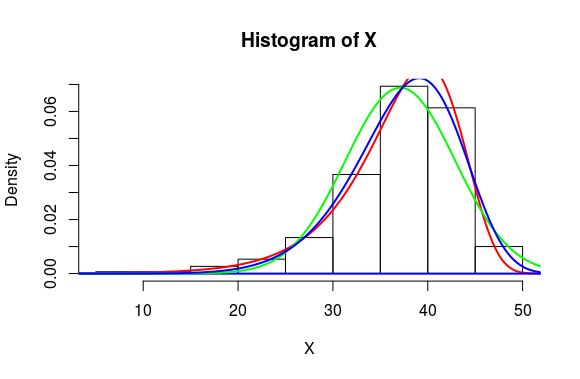
\includegraphics[scale=0.5]{./figures/los3.png}
\caption{SEV(Rojo) vs Weibull(azul) vs Normal(verde)}
\end{figure}
Finalmente si incluimos el caso normal obtenemos los siguientes gráficos donde obtuvimos una normal con $\mu =37.103854$ y $\sigma = 5.803858$\\

% Aqui hay q poner la tabla con los estimados  al hacer el QQ-plot y la recta de ajuste
% Junto con los graficos de probabilidad asociados
\pagebreak
\section*{Parte II}
\begin{enumerate}[a)]
\item La tabla que contiene todas las medidas descriptivas de las variables pedidas es:\\
\begin{figure}[h!]
\begin{adjustwidth}{-2cm}{}
\begin{tabular}{|c|c|c|c|c|c|c|c|c|c|}
\hline
                    &Min.&   1st Qu.&   Median       & Mean&  3rd Qu.&     Max.&          SD   & Skewness&   Kurtosis\\
\hline
Latitud       &   -33.554&  -33.1805&  -33.078 & -33.099476&  -33.017 & -32.416&   0.1269418& -0.09846606 & 1.1670473\\
\hline
Longitud  &       -72.977 & -72.1135&  -72.033 & -72.031659&  -71.942 & -71.517&   0.1442260& -0.57929057&  4.1473745\\
\hline
Magnitud &          2.000  &  2.7000&    3.000   & 3.131190&    3.500&    6.900&   0.6488228 & 1.38533421&  2.8242733\\
\hline
Profundidad    &    2.700 &  20.1000&   24.100  & 24.009439 &  27.300 &  57.100 &  5.7071458 & 0.41369174 & 2.2597913\\
\hline
Radiacion  &        0.000   & 0.0000 &   0.000 & 164.257182 & 184.000 & 813.000& 270.6498715 & 1.34462610 & 0.1144774\\
\hline
Presion  &       1005.000& 1007.0000& 1008.000& 1008.868673& 1010.000 &1014.000  & 2.4274099 & 0.41990366& -0.6890786\\
\hline
Humedad   &        16.000  & 45.0000 &  60.000  & 58.979480&   71.000 &  93.000 & 15.7273295& -0.19424249& -0.9409620\\
\hline
Temperatura   &     7.700  & 12.4000 &  14.600  & 15.632421 &  19.400 &  27.100 &  4.2527190 & 0.49798253& -0.7191210\\
\hline
VelocidadViento  &  0.000 &   0.0000 &   0.500   & 0.773461 &   1.000  &  4.600 &  1.0058630 & 2.16080366 & 4.7130024\\
\hline
\end{tabular}
\end{adjustwidth}
\end{figure}

Los gráficos de las variables serán
\begin{figure}[h!]
\centering
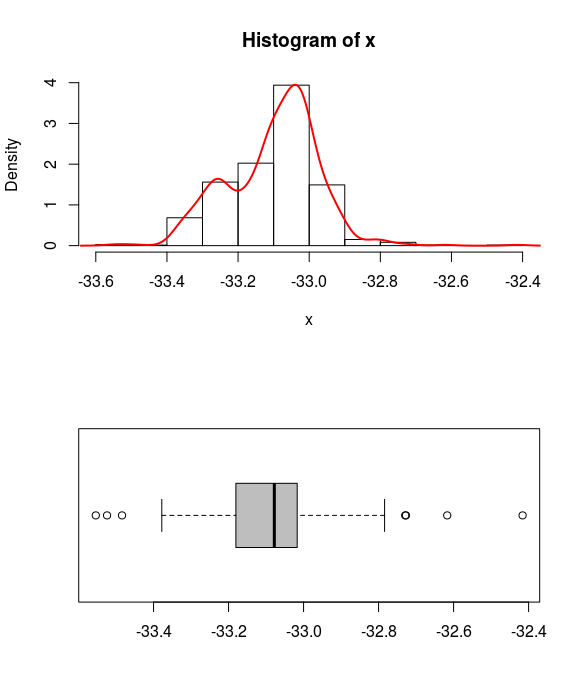
\includegraphics[scale=0.5]{./figures/histplot_Latitud.png}
\caption{Histograma y Boxplot de Latitud}
\end{figure}

\begin{figure}[h!]
\centering
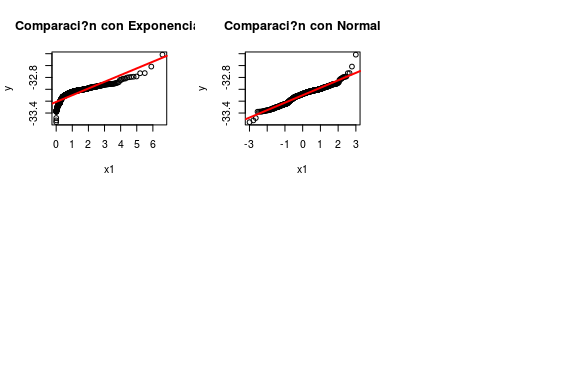
\includegraphics[scale=0.5]{./figures/cm_Latitud.png}
\caption{Comparación con modelos de Latitud}
\end{figure}

\begin{figure}[h!]
\centering
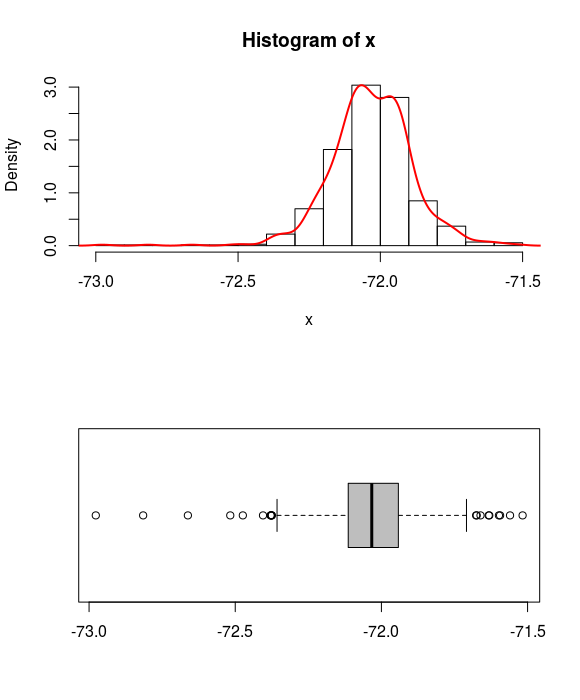
\includegraphics[scale=0.5]{./figures/histplot_Longitud.png}
\caption{Histograma y Boxplot de Longitud}
\end{figure}

\begin{figure}[h!]
\centering
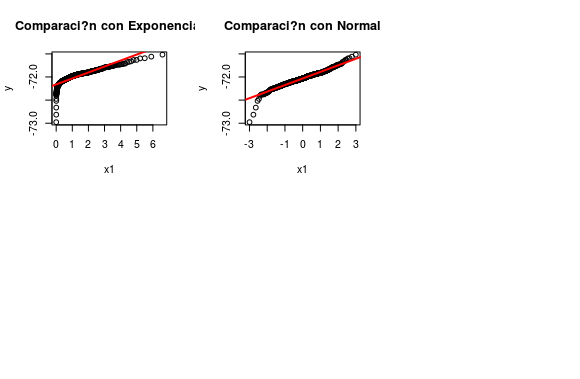
\includegraphics[scale=0.5]{./figures/cm_Longitud.png}
\caption{Comparación con modelos de Longitud}
\end{figure}

\begin{figure}[h!]
\centering
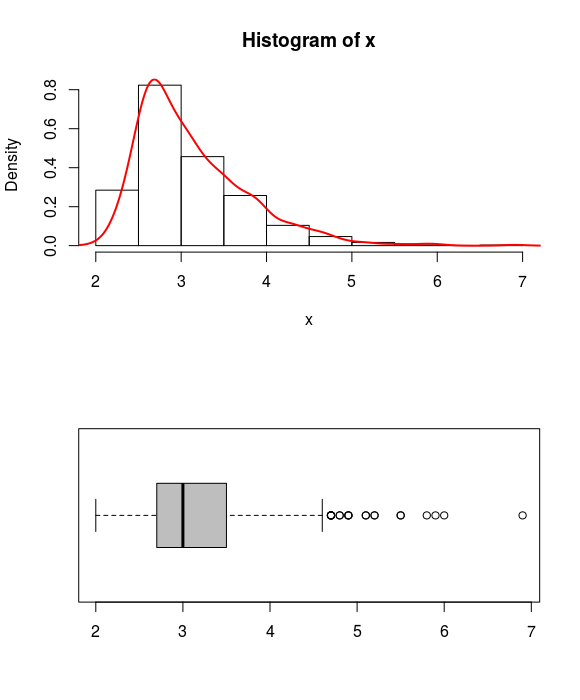
\includegraphics[scale=0.5]{./figures/histplot_Magnitud.png}
\caption{Histograma y Boxplot de Magnitud}
\end{figure}

\begin{figure}[h!]
\centering
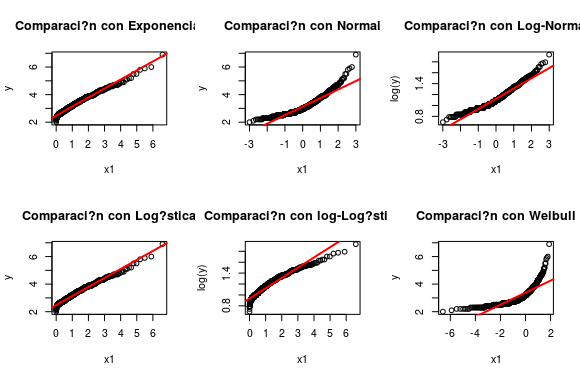
\includegraphics[scale=0.5]{./figures/cm_Magnitud.png}
\caption{Comparación con modelos de Magnitud}
\end{figure}

\begin{figure}[h!]
\centering
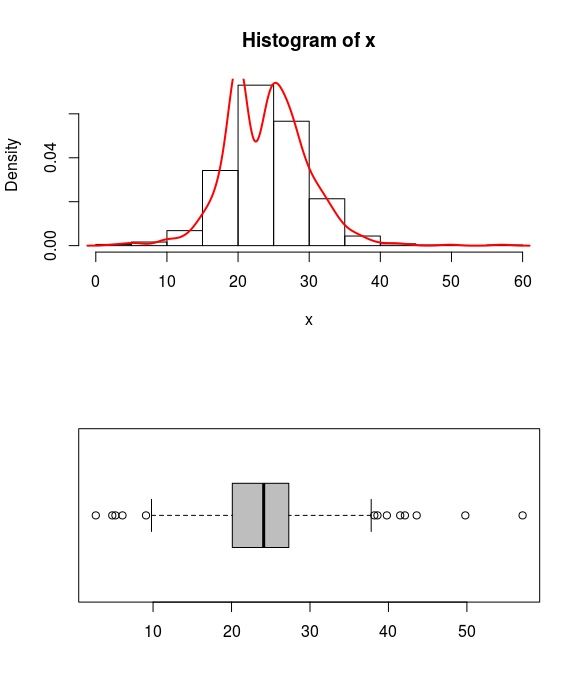
\includegraphics[scale=0.5]{./figures/hisplot_Profundidad.png}
\caption{Histograma y Boxplot de Profundidad}
\end{figure}

\begin{figure}[h!]
\centering
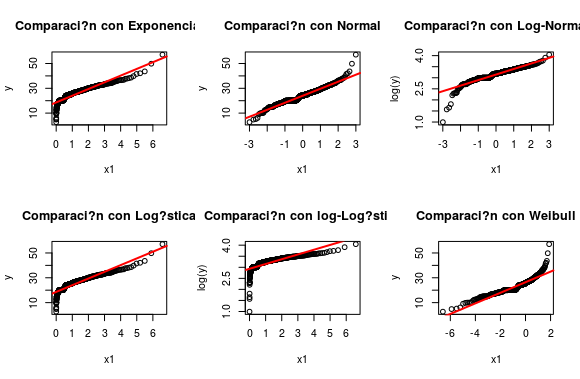
\includegraphics[scale=0.5]{./figures/cm_Profundidad.png}
\caption{Comparación con modelos de Profundidad}
\end{figure}

\begin{figure}[h!]
\centering
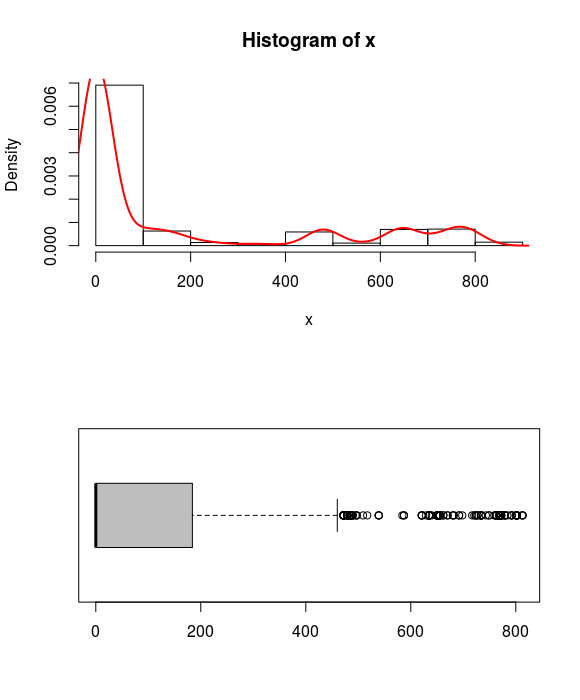
\includegraphics[scale=0.5]{./figures/histplot_Radiacion.png}
\caption{Histograma y Boxplot de Radiacion}
\end{figure}

\begin{figure}[h!]
\centering
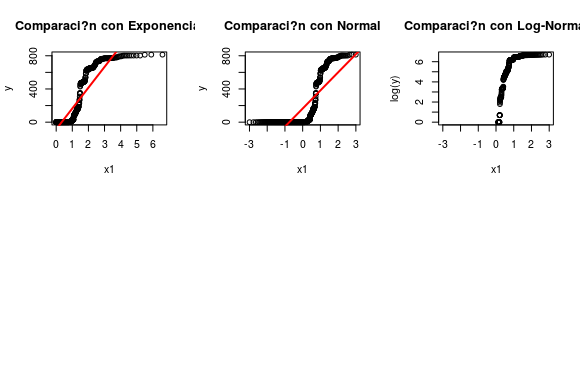
\includegraphics[scale=0.5]{./figures/cm_Radiacion.png}
\caption{Comparación con modelos de Radiacion}
\end{figure}

\begin{figure}[h!]
\centering
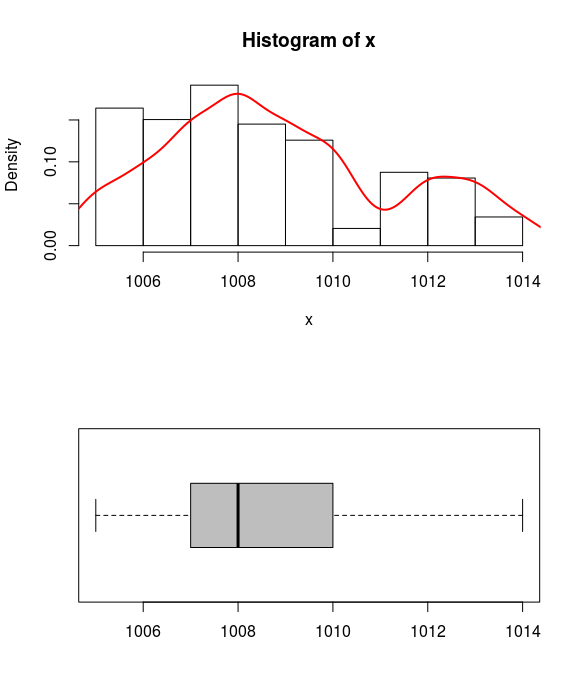
\includegraphics[scale=0.5]{./figures/histplot_Presion.png}
\caption{Histograma y Boxplot de Presion}
\end{figure}

\begin{figure}[h!]
\centering
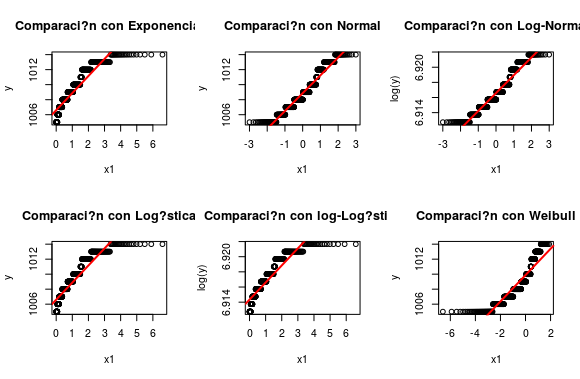
\includegraphics[scale=0.5]{./figures/cm_Presion.png}
\caption{Comparación con modelos de Presion}
\end{figure}

\begin{figure}[h!]
\centering
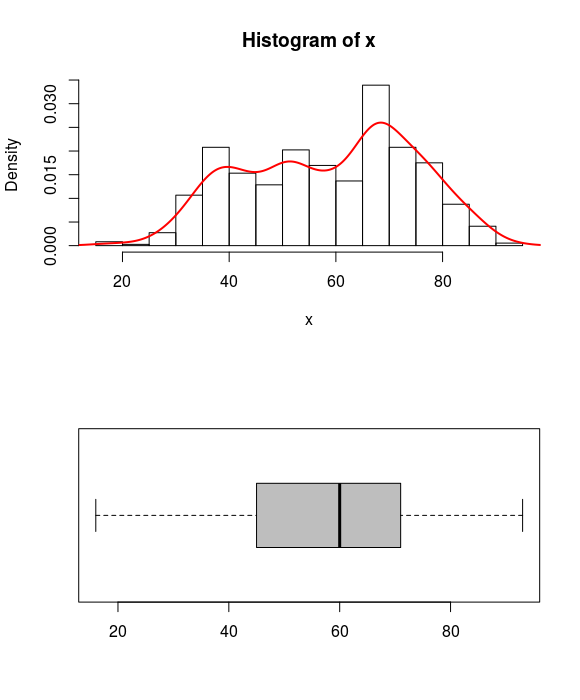
\includegraphics[scale=0.5]{./figures/histplot_Humedad.png}
\caption{Histograma y Boxplot de Humedad}
\end{figure}

\begin{figure}[h!]
\centering
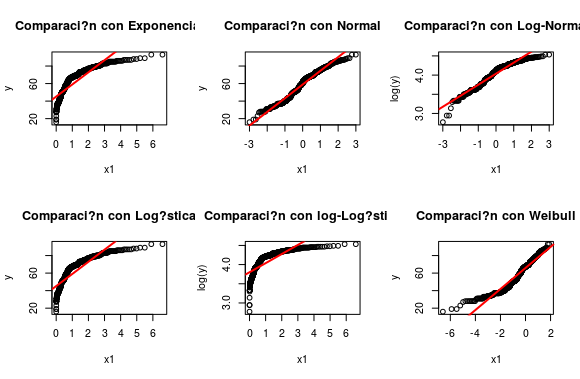
\includegraphics[scale=0.5]{./figures/cm_Humedad.png}
\caption{Comparación con modelos de Humedad}
\end{figure}

\begin{figure}[h!]
\centering
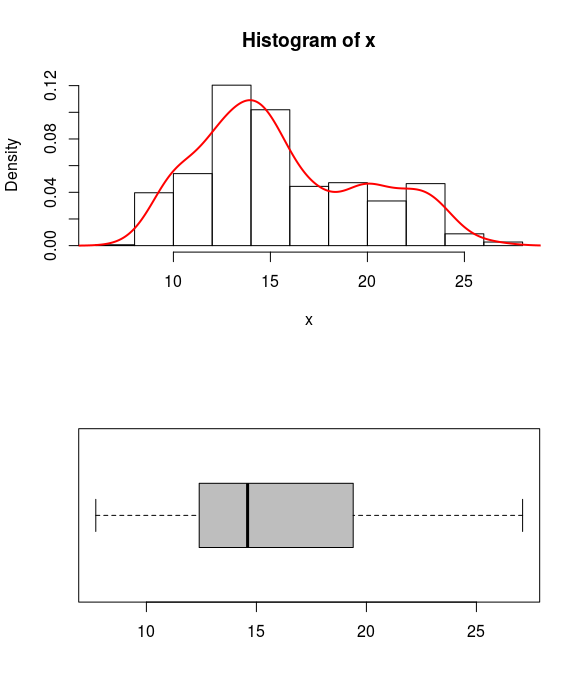
\includegraphics[scale=0.5]{./figures/histplot_Temperartura.png}
\caption{Histograma y Boxplot de Temperatura}
\end{figure}

\begin{figure}[h!]
\centering
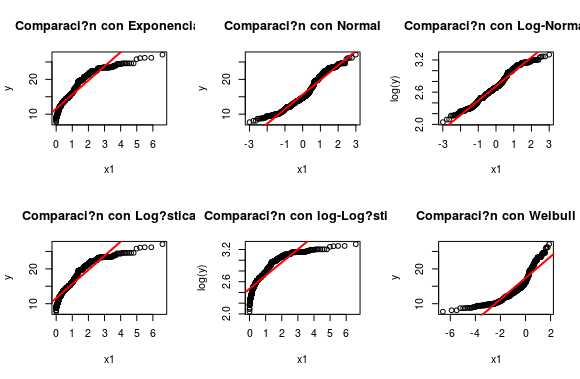
\includegraphics[scale=0.5]{./figures/cm_Temperatura.png}
\caption{Comparación con modelos de Temperatura}
\end{figure}

\begin{figure}[h!]
\centering
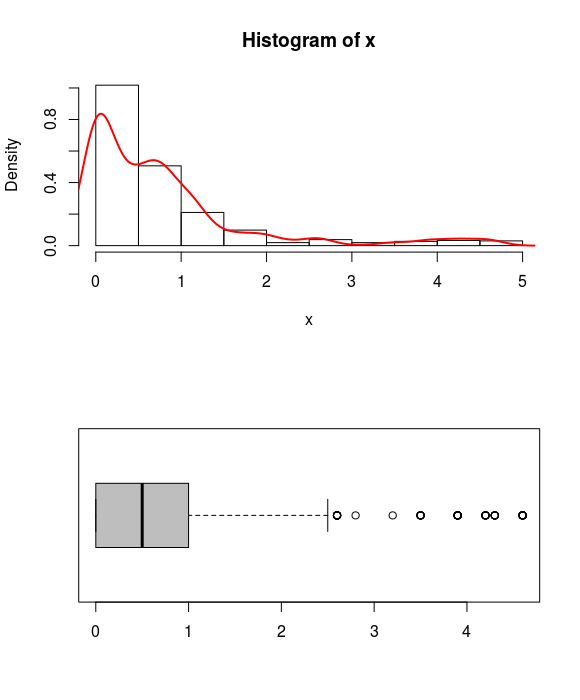
\includegraphics[scale=0.5]{./figures/histplot_Velocidad.png}
\caption{Histograma y Boxplot de Velocidad}
\end{figure}

\begin{figure}[h!]
\centering
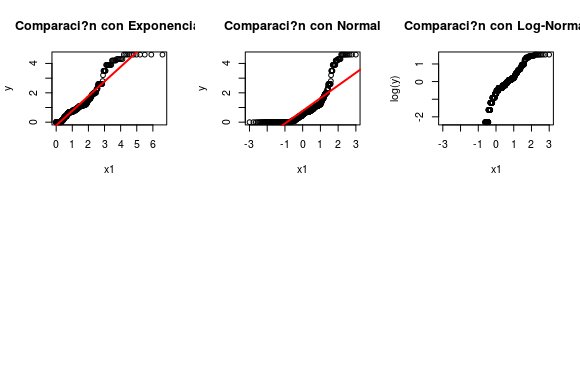
\includegraphics[scale=0.5]{./figures/cm_Velocidad.png}
\caption{Comparación con modelos de Velocidad}
\end{figure}
Hubo un par de gráficos de comparación que no los pude hacer con todas las distribuciones y por temas de tiempo no alcance a obtener todos los parametros de los distintos modelos ajustados a la variables de interes.


 % Describa a partir de medidas empı́ricas y gráficos adecuados las variables: Latitud, Longitud, Magnitud, Profundidad, Radiacion, Presion, Humedad, Temperatura y VelocidadViento, que se encuentran en la Datos02.txt.
\item 20% Represente el comportamiento del número esperado de sismos por hora mediante una función simple con respecto al tiempo u otra variables, desde la ocurrencia del terremoto 6.9 o Richter e ilustre gráficamente. La función lm() y nls() son útiles para estimar coeficientes de funciones lineales y no lineales. El conteo de sismos se encuentra en Datos03.txt.
\end{enumerate}

\end{document}